\documentclass[tikz,border=8pt]{standalone}

\usetikzlibrary{arrows.meta,matrix,fit}

\newlength{\NodeSize}
\newlength{\SiblingDistance}
\newlength{\LevelDistance}
\newlength{\LabelOffset}

\setlength{\NodeSize}{8mm}
\setlength{\SiblingDistance}{12mm}
\setlength{\LevelDistance}{14mm}
\setlength{\LabelOffset}{8mm}

\tikzset{
  tree node/.style={draw, circle, minimum size=\NodeSize, inner sep=0pt},
  array cell/.style={draw, rectangle, minimum width=8mm, minimum height=7mm, inner sep=0pt, align=center, anchor=center},
  label text/.style={draw=none, font=\sffamily\footnotesize},
  index text/.style={draw=none, text=gray, font=\sffamily\scriptsize},
  tree index/.style={draw, fill=white, text=gray, rounded corners=1pt, rectangle, inner sep=1.4pt, font=\sffamily\scriptsize},
  highlight/.style={draw, rounded corners=1pt, inner sep=-1pt}
}

\begin{document}

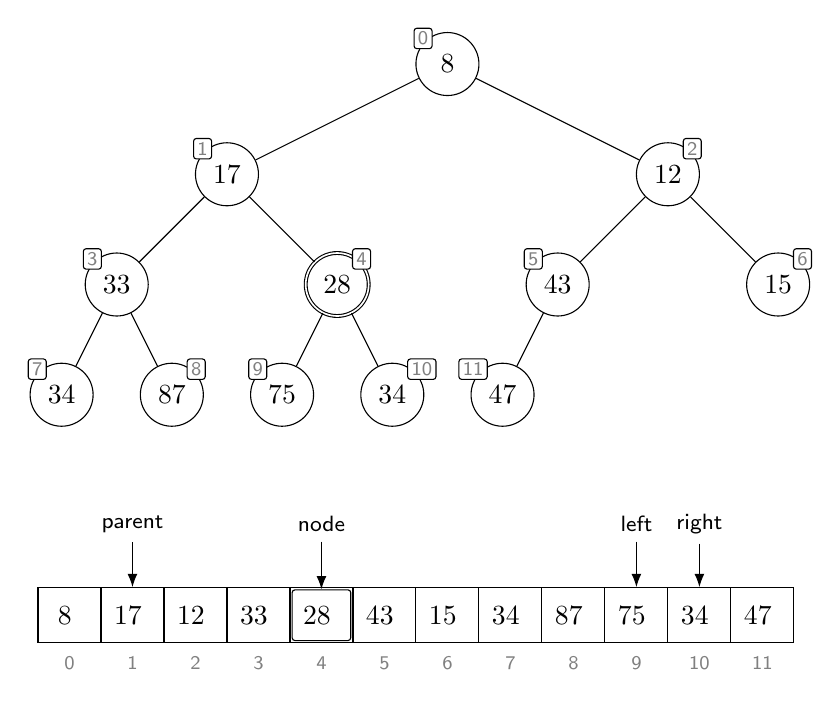
\begin{tikzpicture}[
  >=Latex,
  level distance=\LevelDistance,
  level 1/.style={sibling distance=56mm},
  level 2/.style={sibling distance=28mm},
  level 3/.style={sibling distance=14mm}
]
  \node[tree node] (n8) {8}
    child {
      node[tree node] (n17) {17}
      child {
        node[tree node] (n33) {33}
        child {node[tree node] (n34a) {34}}
        child {node[tree node] (n87) {87}}
      }
      child {
        node[tree node, double] (n28) {28}
        child {node[tree node] (n75) {75}}
        child {node[tree node] (n34b) {34}}
      }
    }
    child {
      node[tree node] (n12) {12}
      child {
        node[tree node] (n43) {43}
        child {node[tree node] (n47) {47}}
        child[missing]
      }
      child {node[tree node] (n15) {15}}
    };

  \node[tree index, anchor=south east] at ([xshift=1mm,yshift=-1mm]n8.north west) {0};
  \node[tree index, anchor=south east] at ([xshift=1mm,yshift=-1mm]n17.north west) {1};
  \node[tree index, anchor=south west] at ([xshift=-1mm,yshift=-1mm]n12.north east) {2};
  \node[tree index, anchor=south east] at ([xshift=1mm,yshift=-1mm]n33.north west) {3};
  \node[tree index, anchor=south west] at ([xshift=-1mm,yshift=-1mm]n28.north east) {4};
  \node[tree index, anchor=south east] at ([xshift=1mm,yshift=-1mm]n43.north west) {5};
  \node[tree index, anchor=south west] at ([xshift=-1mm,yshift=-1mm]n15.north east) {6};
  \node[tree index, anchor=south east] at ([xshift=1mm,yshift=-1mm]n34a.north west) {7};
  \node[tree index, anchor=south west] at ([xshift=-1mm,yshift=-1mm]n87.north east) {8};
  \node[tree index, anchor=south east] at ([xshift=1mm,yshift=-1mm]n75.north west) {9};
  \node[tree index, anchor=south west] at ([xshift=-1mm,yshift=-1mm]n34b.north east) {10};
  \node[tree index, anchor=south east] at ([xshift=1mm,yshift=-1mm]n47.north west) {11};

  \matrix (arr) [
    matrix of nodes,
    nodes={array cell},
    column sep=-\pgflinewidth,
    row sep=-\pgflinewidth,
    anchor=center
  ] at (-0.4,-7.0) {
    8 & 17 & 12 & 33 & 28 & 43 & 15 & 34 & 87 & 75 & 34 & 47 \\
  };

  \foreach \i in {1,...,12} {
    \pgfmathtruncatemacro{\idx}{\i-1}
    \node[index text] at ([yshift=-2.5mm]arr-1-\i.south) {\idx};
  }

  \node[label text] (labparent) at ([yshift=\LabelOffset]arr-1-2.north) {parent};
  \node[label text] (labnode)   at ([yshift=\LabelOffset]arr-1-5.north) {node};
  \node[label text] (lableft)   at ([yshift=\LabelOffset]arr-1-10.north) {left};
  \node[label text] (labright)  at ([yshift=\LabelOffset]arr-1-11.north) {right};

  \node[highlight, fit=(arr-1-5)] (hnode) {};

  \draw[-Latex] (labparent.south) -- (arr-1-2.north);
  \draw[-Latex] (labnode.south) -- (hnode.north);
  \draw[-Latex] (lableft.south) -- (arr-1-10.north);
  \draw[-Latex] (labright.south) -- (arr-1-11.north);
  % \draw[-Latex] (labnode.north) to[out=90,in=-60] (n28.south);
\end{tikzpicture}
\end{document}
